\section{Student}
\subsection{Progress Tracking}
Hệ thống theo dõi tiến độ học tập được thiết kế để giúp sinh viên nắm rõ quá trình học tập của họ trong khóa học.
\begin{itemize}
    \item Thông tin khóa học cơ bản
    \begin{itemize}
        \item Chi tiết khóa học.
        \item Tiến độ hoàn thành.
        \item Mục tiêu sinh viên trong khóa học.
        \item Learning Outcomes
    \end{itemize}
    \begin{figure}[H]
        \centering
        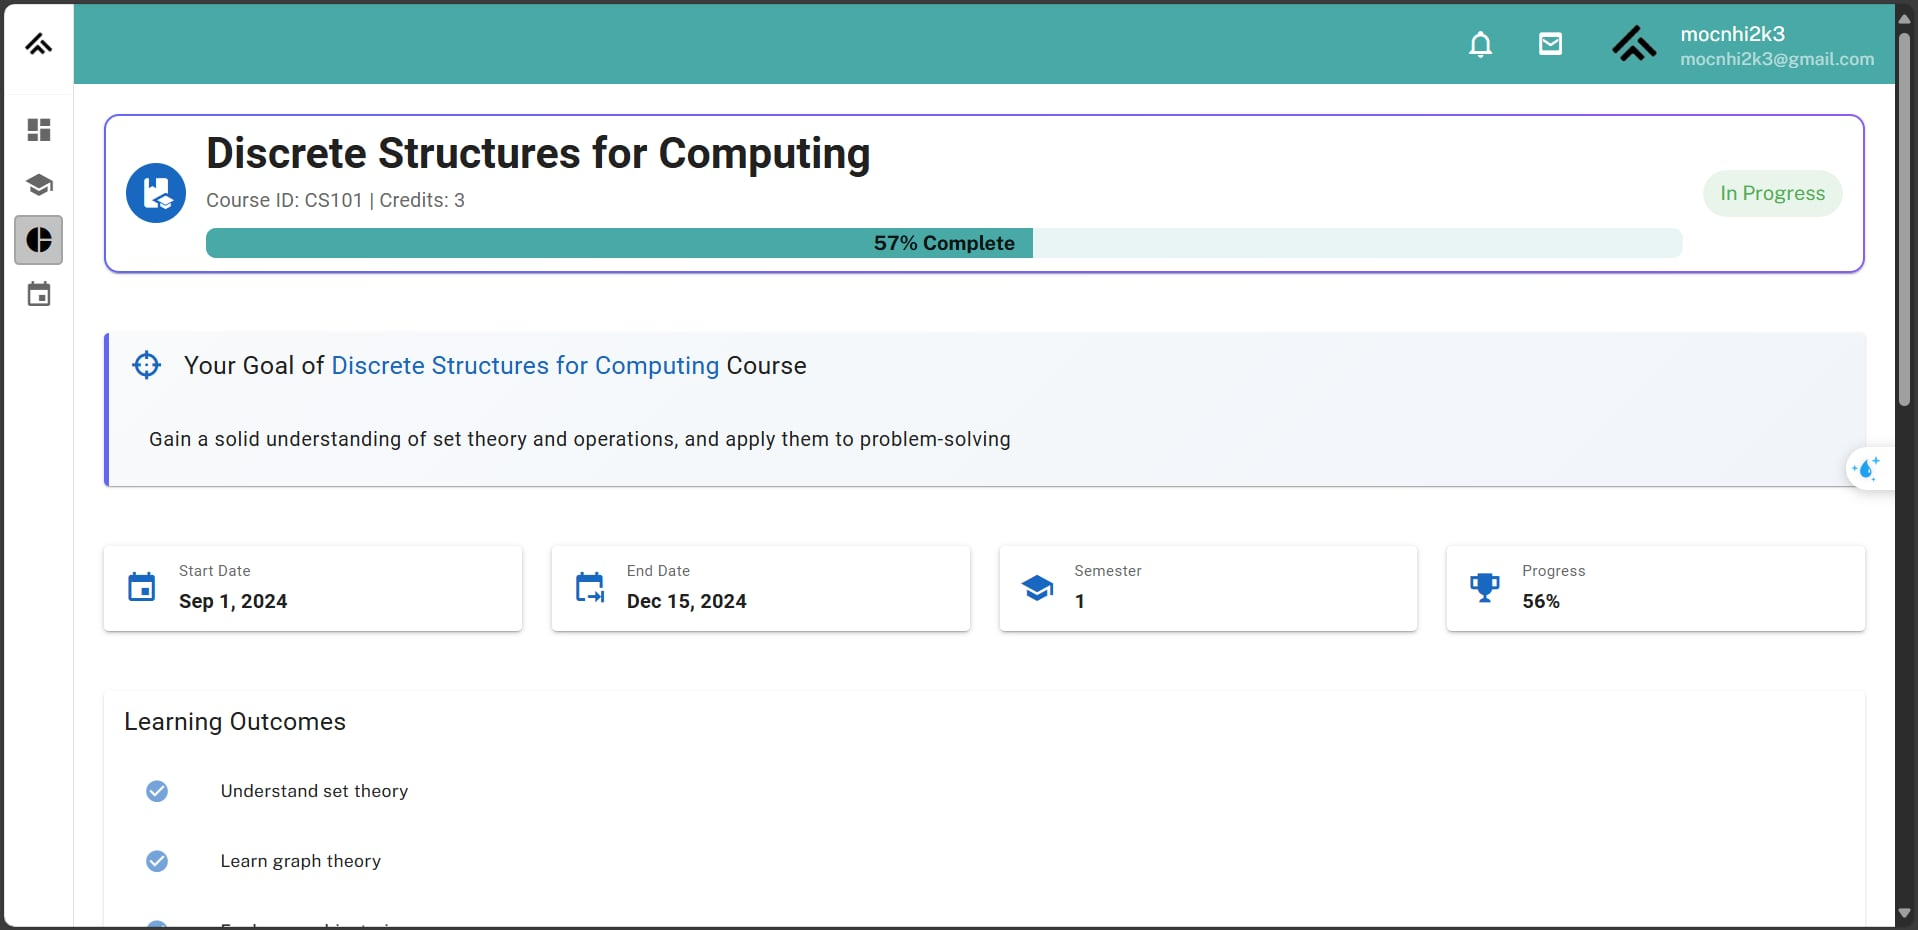
\includegraphics[width=0.8\linewidth]{images/progress_info_course.png}
        \caption{Thông tin khóa học}
        \label{fig:enter-label}
    \end{figure}
    \item Performance Metrics:
    \begin{itemize}
        \item Tỷ lệ hoàn thành bài tập
        \item Điểm số trung bình
        \item Thời gian học tập
        \item Mức độ tương tác với nội dung khóa học
    \end{itemize}
    \begin{figure}[H]
        \centering
        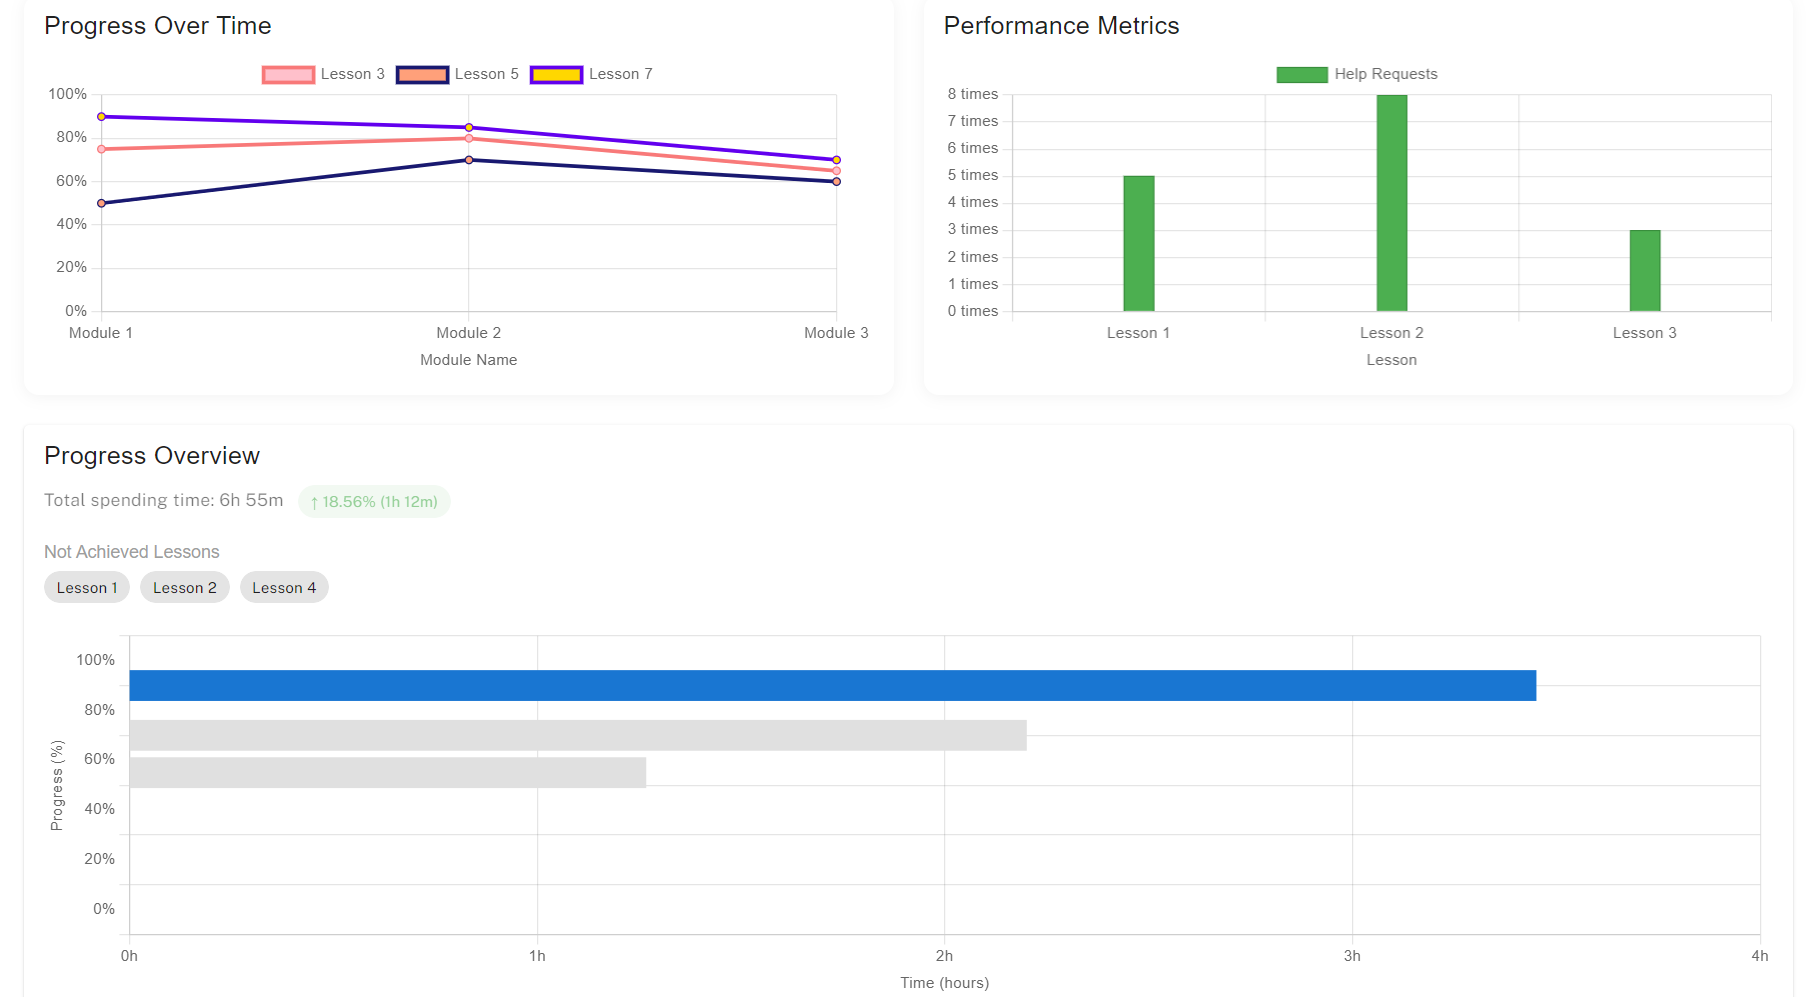
\includegraphics[width=0.8\linewidth]{images/progress_statistic.png}
        \caption{Thống kê kết quả học tập}
        \label{fig:enter-label}
    \end{figure}
\end{itemize}
